\section{Estudio Experimental}

\subsection{Metodología y Entorno de Pruebas}

Los experimentos se ejecutaron en un equipo con sistema operativo Windows 11 Home,
compilando con MinGW-w64 GCC 14.x en modo Release (optimización \texttt{-O2}).
Cada métrica se ejecutó \textbf{10 veces consecutivas} sobre el grafo ya construido
en memoria, reportando media aritmética, varianza, mínimo y máximo. La medición de
tiempo utiliza \texttt{std::chrono::high\_resolution\_clock}.

El código fuente está disponible en:
\url{https://github.com/ricachii/Centralidad-de-Redes}

\subsection{Construcción del Grafo}

\begin{center}
\begin{tabular}{lcc}
\toprule
\textbf{Dataset} & \textbf{Tiempo de construcción (ms)} & \textbf{Memoria (KB)} \\
\midrule
Yeast PPI (6.526V, 532.180E) & 3.902 & 24.150 \\
Trade Network (161V, 22.475E) & 551 & 571 \\
\bottomrule
\end{tabular}
\end{center}

La diferencia de memoria (24 MB vs 571 KB) refleja directamente el tamaño de cada red.
Usando lista de adyacencia, Yeast ocupa $\sim$24 MB frente a los $\sim$340 MB que
requeriría una matriz de adyacencia ($6.526^2$ entradas).

\subsection{Tiempo de Ejecución por Métrica}

\subsubsection*{Dataset 1: Yeast PPI}

\begin{center}
\begin{tabular}{lcccc}
\toprule
\textbf{Métrica} & \textbf{Media (ms)} & \textbf{Varianza (ms$^2$)} & \textbf{Mín} & \textbf{Máx} \\
\midrule
Degree Centrality     & 0{,}73      & 0{,}007    & 0{,}641   & 0{,}923  \\
PageRank              & 298         & 177        & 290       & 337      \\
Eigenvector           & 411         & 178        & 404       & 451      \\
Clustering Coeff.     & 10.493      & 341        & 10.459    & 10.514   \\
Closeness             & 60.020      & 3.365      & 59.903    & 60.128   \\
Average Shortest Path & 60.042      & 4.577      & 59.964    & 60.158   \\
Betweenness           & 109.452     & 87.823     & 109.039   & 110.020  \\
\bottomrule
\end{tabular}
\end{center}

\subsubsection*{Dataset 2: Trade Network}

\begin{center}
\begin{tabular}{lcccc}
\toprule
\textbf{Métrica} & \textbf{Media (ms)} & \textbf{Varianza (ms$^2$)} & \textbf{Mín} & \textbf{Máx} \\
\midrule
Degree Centrality     & 0{,}025 & $1{,}5\times10^{-5}$ & 0{,}020 & 0{,}032 \\
PageRank              & 24{,}9  & 0{,}18               & 24{,}3  & 25{,}7  \\
Eigenvector           & 34{,}5  & 0{,}049              & 34{,}3  & 34{,}9  \\
Clustering Coeff.     & 699     & 581                  & 666     & 727     \\
Closeness             & 705     & 735                  & 673     & 739     \\
Average Shortest Path & 702     & 644                  & 672     & 737     \\
Betweenness           & 722     & 1.602                & 647     & 786     \\
\bottomrule
\end{tabular}
\end{center}

\begin{figure}[h]
\centering
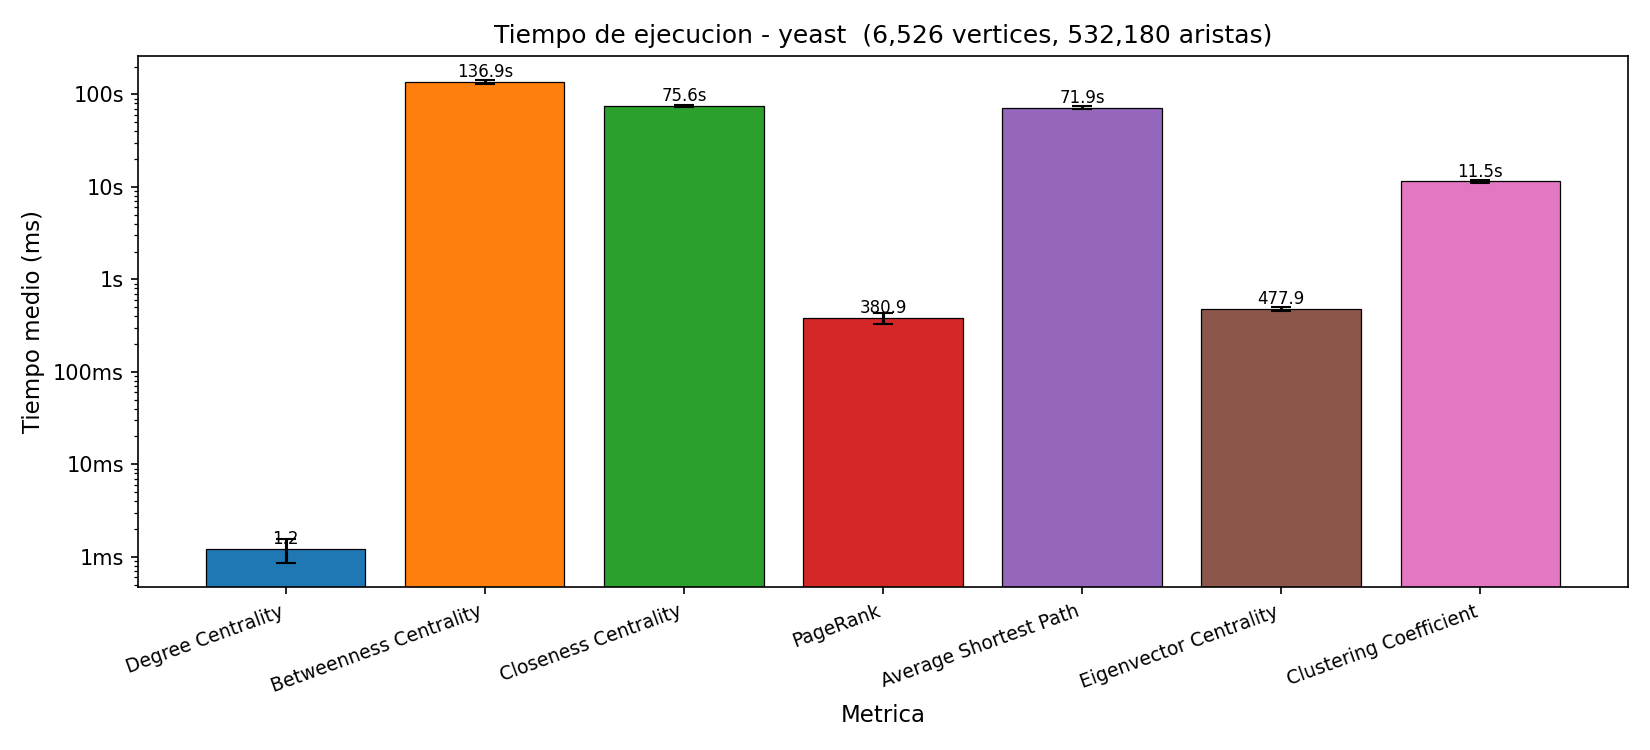
\includegraphics[width=0.48\textwidth]{../results/plots/yeast_tiempos.png}
\hfill
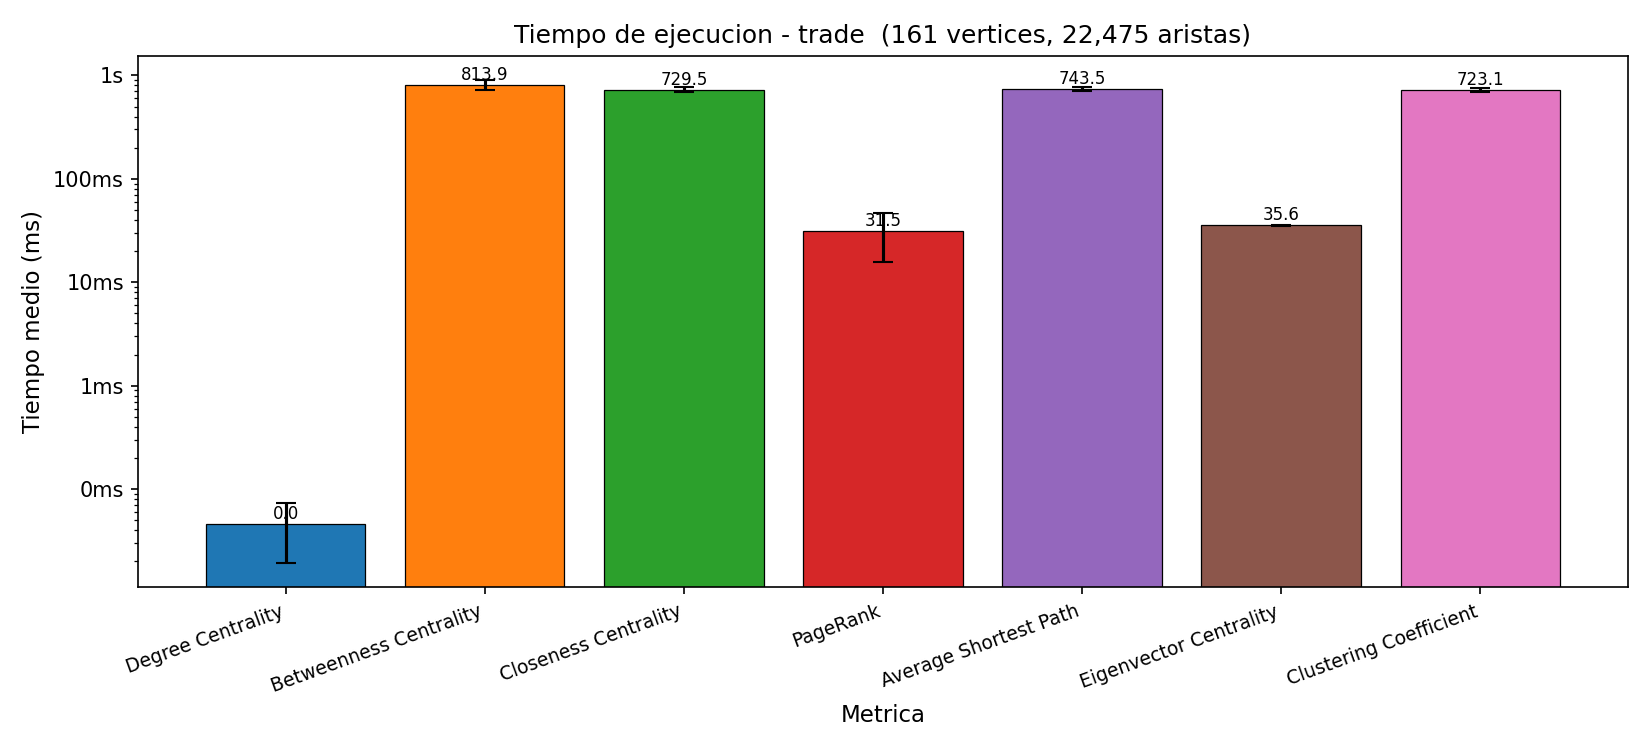
\includegraphics[width=0.48\textwidth]{../results/plots/trade_tiempos.png}
\caption{Tiempos de ejecución por métrica. Izquierda: Yeast PPI. Derecha: Trade Network.
Escala logarítmica para visualizar el rango de 6 órdenes de magnitud.}
\end{figure}

\subsection{Métricas Adicionales: Eigenvector y Clustering Coefficient}

\textbf{Eigenvector Centrality} tardó 411 ms en Yeast (varianza 178 ms$^2$) y 34,5 ms
en Trade (varianza 0,049 ms$^2$). La baja varianza en ambos datasets confirma que
Power Iteration converge de forma predecible en menos de 100 iteraciones.
En Yeast, los nodos con alta Eigenvector Centrality corresponden a proteínas que
interactúan con otras proteínas también muy conectadas, formando el núcleo funcional
de la red. En Trade, identifica países cuya influencia comercial se amplifica a través
de sus socios estratégicos.

\textbf{Clustering Coefficient} tardó 10.493 ms en Yeast (varianza 341 ms$^2$) y
699 ms en Trade (varianza 581 ms$^2$). La varianza es la más baja de las métricas
lentas, producto del comportamiento determinista del conteo de triángulos.
En Yeast, el alto coeficiente de clustering global indica la presencia de complejos
proteicos: módulos donde todas las proteínas interactúan entre sí (ribosomas, complejos
de transcripción). En Trade, países con alto clustering pertenecen a bloques comerciales
regionales donde sus socios también comercian entre sí.

\subsection{Impacto de Modificaciones Estructurales}

Se evaluó el impacto de agregar y quitar 5 aristas en tres zonas: nodos \textit{hub}
(top 10\% por grado), periféricos (bottom 10\%) y posiciones aleatorias.

\subsubsection*{Yeast PPI}

\begin{center}
\begin{tabular}{llccc}
\toprule
\textbf{Op.} & \textbf{Zona} & \textbf{Betweenness} & \textbf{Closeness} & \textbf{ASP} \\
\midrule
$+$5 & Hub        & $-4{,}3\times10^{-5}$\% & $+2{,}5\times10^{-5}$\% & $-2{,}3\times10^{-5}$\% \\
$+$5 & Periférico & $-0{,}007$\%             & $+0{,}003$\%             & $-0{,}004$\% \\
$+$5 & Aleatorio  & $-0{,}001$\%             & $+0{,}0004$\%            & $-0{,}0005$\% \\
\midrule
$-$5 & Hub        & $+5{,}0\times10^{-5}$\% & $-2{,}8\times10^{-5}$\% & $+2{,}8\times10^{-5}$\% \\
$-$5 & Periférico & $-0{,}158$\%             & $-0{,}060$\%             & $-0{,}082$\% \\
$-$5 & Aleatorio  & $-0{,}053$\%             & $-0{,}020$\%             & $-0{,}027$\% \\
\bottomrule
\end{tabular}
\end{center}

\subsubsection*{Trade Network}

\begin{center}
\begin{tabular}{llccc}
\toprule
\textbf{Op.} & \textbf{Zona} & \textbf{Betweenness} & \textbf{Closeness} & \textbf{ASP} \\
\midrule
$+$5 & Hub        & $0$\%        & $0$\%        & $0$\%      \\
$+$5 & Periférico & $+5{,}86$\%  & $+0{,}354$\% & $+1{,}135$\% \\
$+$5 & Aleatorio  & $-0{,}189$\% & $+0{,}013$\% & $-0{,}018$\% \\
\midrule
$-$5 & Hub        & $+0{,}189$\% & $-0{,}021$\% & $+0{,}018$\% \\
$-$5 & Periférico & $+0{,}189$\% & $-0{,}010$\% & $+0{,}018$\% \\
$-$5 & Aleatorio  & $+0{,}189$\% & $-0{,}017$\% & $+0{,}018$\% \\
\bottomrule
\end{tabular}
\end{center}

\subsection{Análisis de los Resultados}

\textbf{Betweenness domina en tiempo.} En Yeast tardó 109 segundos por ejecución,
representando más del 98\% del tiempo total del experimento. Esto confirma la
predicción teórica de $O(|V| \cdot |E|) \approx 3{,}47\times10^9$ operaciones.
El algoritmo de Brandes es indispensable: sin él, la complejidad naive
$O(|V|^2 \cdot |E|)$ haría el cálculo inviable.

\textbf{Closeness y ASP son equivalentes en tiempo.} Ambas realizan BFS desde
cada vértice, compartiendo la implementación \texttt{bfsDistances()}, lo que se
refleja en tiempos casi idénticos (60.020 ms vs 60.042 ms en Yeast).

\textbf{Diferencia de escala entre datasets.} Betweenness en Trade (722 ms) vs
Yeast (109.452 ms) — una diferencia de $\sim$150$\times$, consistente con la
relación entre sus tamaños ($|V|\cdot|E|$: Trade $\approx 3{,}6\times10^6$ vs
Yeast $\approx 3{,}5\times10^9$).

\textbf{Yeast es robusta ante cambios locales.} Con 532.180 aristas, agregar o
quitar 5 produce variaciones menores al 0,2\% en todas las métricas. Los cambios
son mayores en nodos periféricos que en hubs, ya que los hubs ya disponen de
múltiples caminos alternativos.

\textbf{Trade es sensible en su periferia.} Agregar 5 aristas desde nodos
periféricos aumenta Betweenness un 5,86\%, pues crea caminos mínimos nuevos que
reorganizan el flujo global. Los hubs, en cambio, muestran 0\% de cambio al agregar
aristas: con densidad $\approx 87\%$, ya no existen pares sin conexión entre los
nodos más conectados.
